\documentclass{tufte-handout}

\title{On ultimate 2. Using space, using players}
\author[James Reynolds]{James Reynolds}

%\date{28 March 2010} % without \date command, current date is supplied

%\geometry{showframe} % display margins for debugging page layout

\usepackage{graphicx} % allow embedded images
  \setkeys{Gin}{width=\linewidth,totalheight=\textheight,keepaspectratio}
  \graphicspath{{graphics/}} % set of paths to search for images
\usepackage{amsmath}  % extended mathematics
\usepackage{booktabs} % book-quality tables
\usepackage{units}    % non-stacked fractions and better unit spacing
\usepackage{multicol} % multiple column layout facilities
\usepackage{lipsum}   % filler text
\usepackage{fancyvrb} % extended verbatim environments
  \fvset{fontsize=\normalsize}% default font size for fancy-verbatim environments

% Standardize command font styles and environments
\newcommand{\doccmd}[1]{\texttt{\textbackslash#1}}% command name -- adds backslash automatically
\newcommand{\docopt}[1]{\ensuremath{\langle}\textrm{\textit{#1}}\ensuremath{\rangle}}% optional command argument
\newcommand{\docarg}[1]{\textrm{\textit{#1}}}% (required) command argument
\newcommand{\docenv}[1]{\textsf{#1}}% environment name
\newcommand{\docpkg}[1]{\texttt{#1}}% package name
\newcommand{\doccls}[1]{\texttt{#1}}% document class name
\newcommand{\docclsopt}[1]{\texttt{#1}}% document class option name
\newenvironment{docspec}{\begin{quote}\noindent}{\end{quote}}% command specification environment

\begin{document}

\maketitle% this prints the handout title, author, and date

%\printclassoptions

Welcome to (Reynolds) on ultimate, 
a series of two-pagers 
about strategy and tactics for playing frisbee. 
There's a lot to learn\footnote{And plenty of opinions. 
These are mine, but you can always fork the github repository 
(https://github.com/James-Reynolds/Ultimate-strategy-and-tactics)
or make a pull request if you want to put yours to paper.}, 
and explaining stuff
on the field or at trainings
can be challenging.  
These notes 
aim to be a written resource 
instead. 
This is the second note, focusing on horizontal and vertical offensive structures 
(against person-match defence) 
and offense against 3-3-1 and 2-3-2 zone structures\footnote{They obviously simplify everything as much as possible.
For example: the force is assumed to be forehand unless otherwise stated;  
O1-4 are the cutters, O5-7 are the handlers, D8-14 are on defence; 
Offence is always going down the page (the enemy's gate...). Some prior knowledge is assumed.}. 



\newthought{Each possession} 
might end in: 
1) a score\footnote{Then pulling to the other team to start the next point.}; 
2) a turnover because of defensive actions (a 'D', stall out, forced error, etc.); or 
3) a turnover through unforced error ('throwaway', 'cold drop' etc.).
The difference in score
is related to the difference 
in turnovers.  
Probability of a turnover instead of a score 
is a function of 
the number of passes made 
prior to scoring 
and the pass completion rate.
Hence, fewer passes\footnote{
One throw to the endzone, with a 50\% chance of completion...} 
and/or higher completion rates\footnote{
...versus five throws
to score, 
each with a completion rate of 90\% 
(total 59\%) or only 85\%  
(total 44\%).}  
might be preferred. 

Reality is more complex, 
with
completion rates 
varying by 
thrower, 
receiver, 
throw 
and situation\footnote{Plus 
\smallcaps{second-order factors},  
where someone 
takes bigger risks 
because a turnover is 
likely anyway.}.
There's a balance 
to be found,
%\footnote{The possession/territory
%dilemma is common in many sports. 
%But, unless it is really windy,
%ultimate seems weighted 
%more towards possession. 
%You have ten seconds 
%to pass it (unlike netball's three). 
%The field is huge and
%there's only seven people on each team 
%(just like rugby 7s, but more so because there's no tackling!)}, 
 but if you receive the pull 
 the 'desired' result is  
 retaining possession until you
 score\footnote{A 'clean hold'}, 
 the 'neutral' result is to score despite 
 losing possession at least once\footnote{A 'hold', but an opportunity given to them to score instead} while the 'bad' outcome  
 is they score and you receiving the pull again next point\footnote{"Defence wins games. Offence loses them". Old handler proverb (probably)}.

\newthought{Defence sets the agenda; offense responds to it}:
Defend each person individually ('person-match')
and throwing into space may be easier;
Covering space instead ('zone', 'clam' or 'junk') may leave open throws to unmarked people, 
but delay downfield progress;
Forcing forehand makes backhands harder; 
Forcing 'straight up' makes it harder to throw long 
and to the centre of the field; 
Covering 'deep' likewise makes long throws harder; and so on. 

\begin{marginfigure}%
  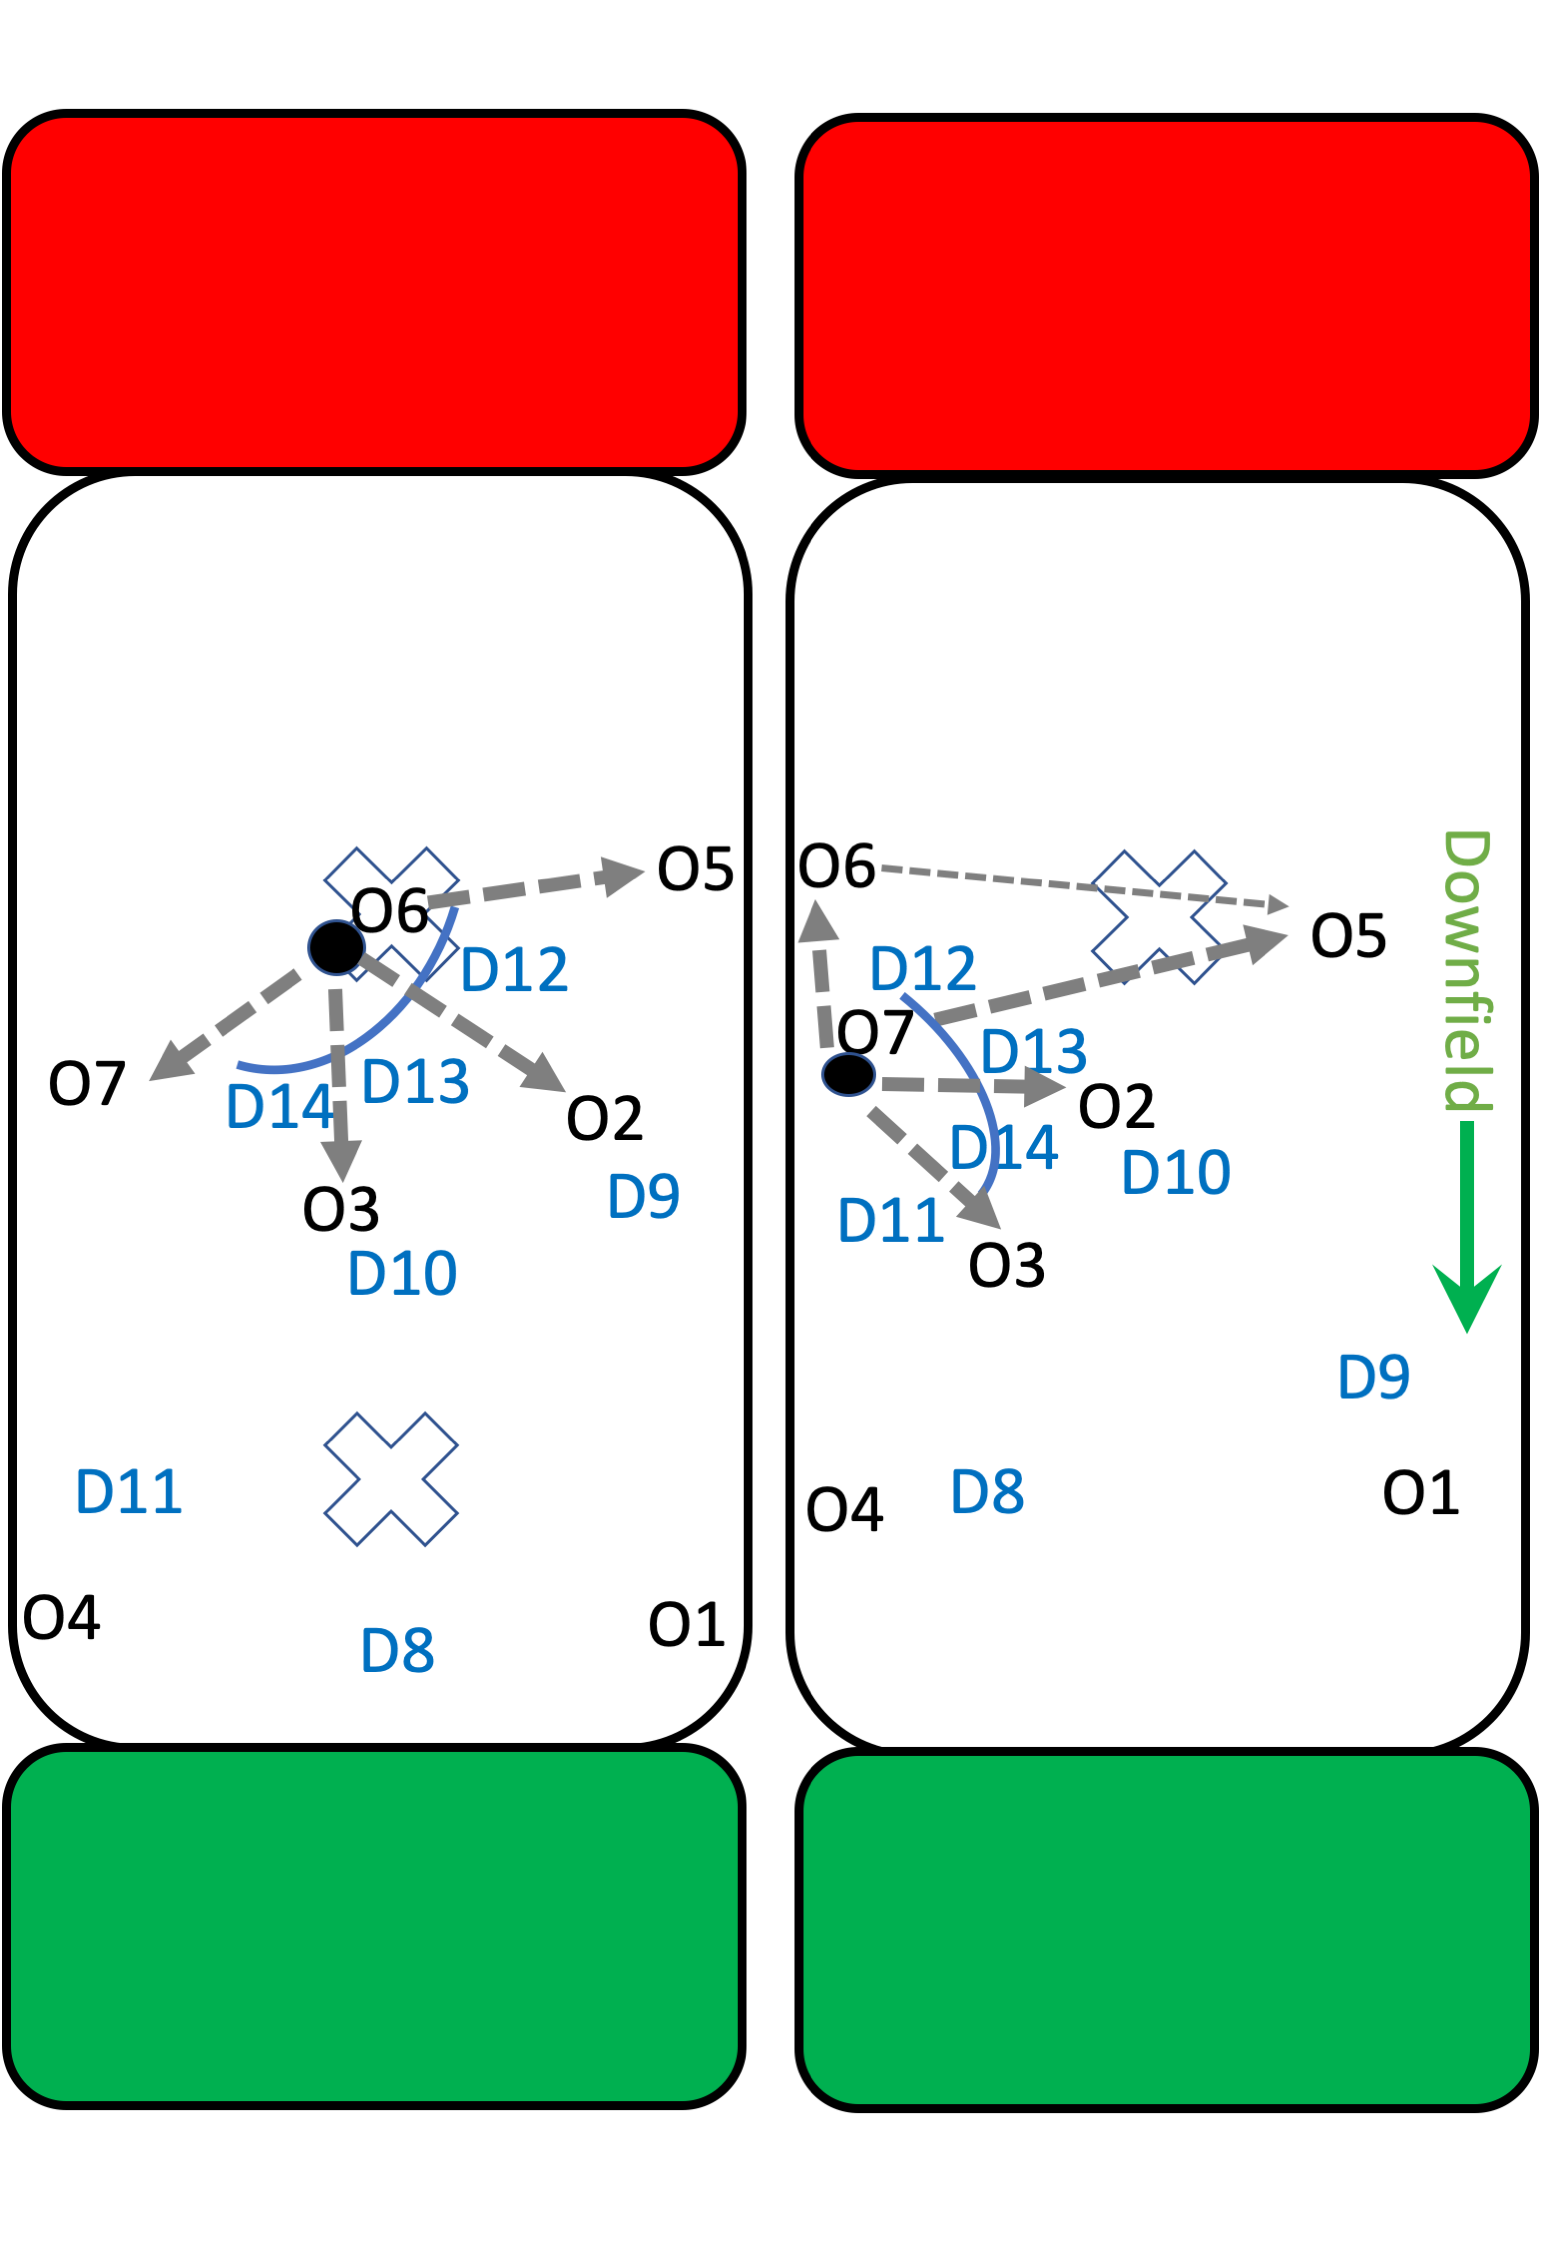
\includegraphics[width=\linewidth]{dump_zone}
 \caption{3-3-1 zone}
 \label{fig:dump_zone}
 \end{marginfigure}

Figure 1 shows a 3-3-1 zone\footnote{The first 3 are D12,13 and 14 (the cup, limiting downfield throws, often forcing throws to go over or around the cup)). 
The second 3 are limiting movement (around) to the wings (D9, 11) or (over) to the 'middle middle' or 'short deep' (D10), 
while the 1 is D8 limiting the ' deep deep' throws downfield)}, 
which might make throws amongst the handlers 
(O5, 6 and 7) easier as they are unmarked,
but make throws to downfield players
(O1-4) more challenging.  
But what happens once you get the disc 
to someone downfield, say O3? 
Until D12-14 arrive (Figure 2, left) it might be 
two (O4, O1)-versus-two(D8 and D11 or 9) 
downfield of the disc, 
suggesting more progress 
towards the endzone may be relatively easy. 
 Once D12-14 arrive, however (Figure 2, right), 
the cup reforms and downfield receivers are outnumbered. 
It is probably time for O3 to 'dump' 
back to an unmarked handler (O5-7), 
get downfield and 
be a receiver again.  

\begin{marginfigure}%
  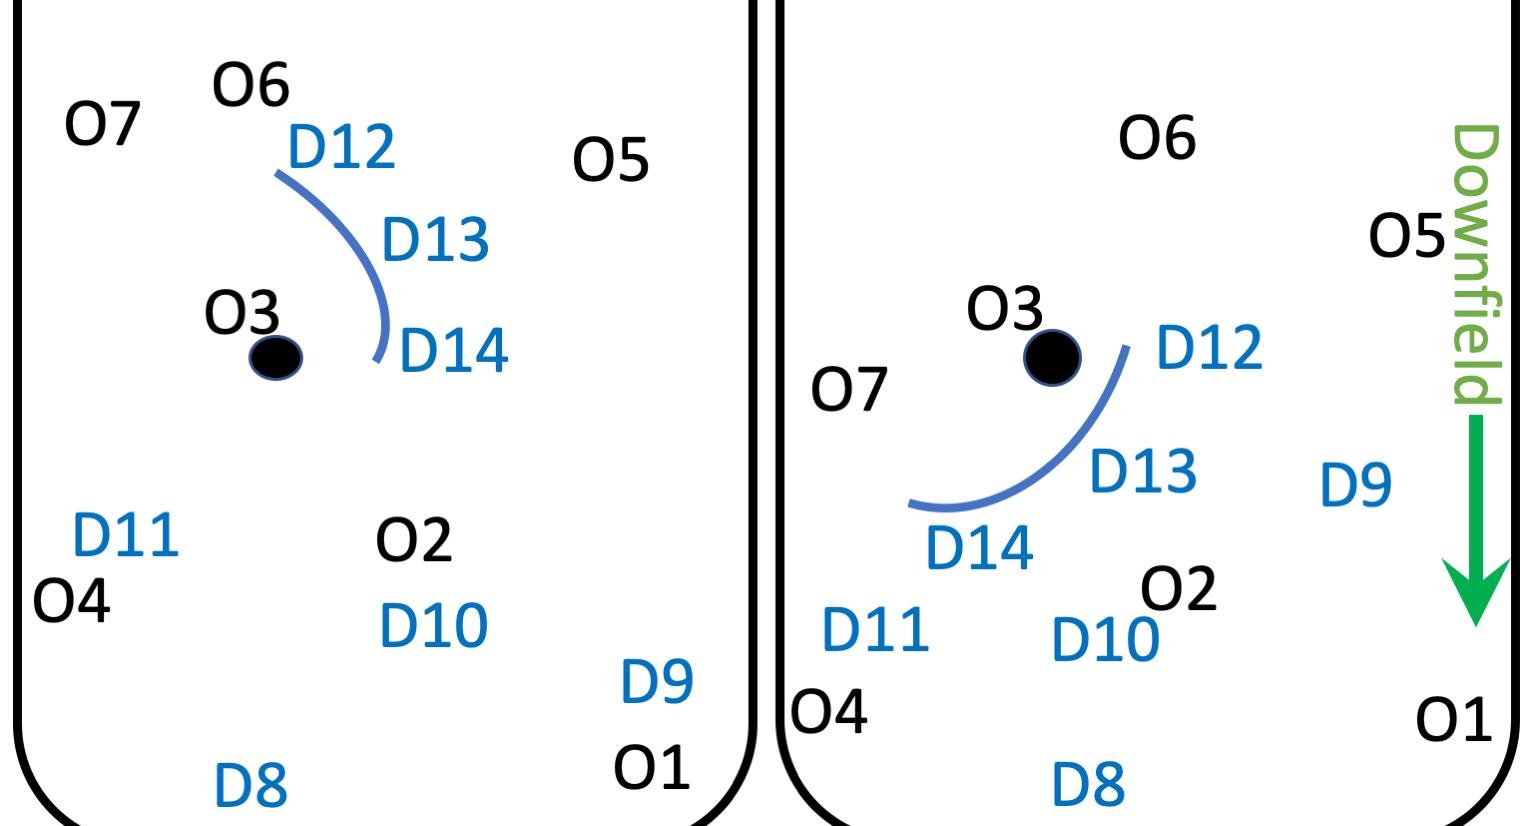
\includegraphics[width=\linewidth]{dump_zone2}
 \caption{3-3-1, with O3 before (left) and after (right) the cup catches up}
 \label{fig:dump_zone2}
 \end{marginfigure}

\newthought{When to dump} 
might depend on your role\footnote{If you are a cutter, 
probably dump 
and run ASAP.   
Get it back to the handlers 
and they'll throw it to you again!}. 
As well, against person-match defence it 
might take a while to get a dump off.  
One rule of thumb is to look to dump from stall 4 or 5 until 8 or so
\footnote{Then huck for position on 9}. 
That said, defenders might give you an early dump 
so as to 'poach',
as in Figure \ref{fig:dump_match_1_45}(left) where 
D14 is preventing downfield progress rather than matching 
up on O7. 

\begin{marginfigure}%
  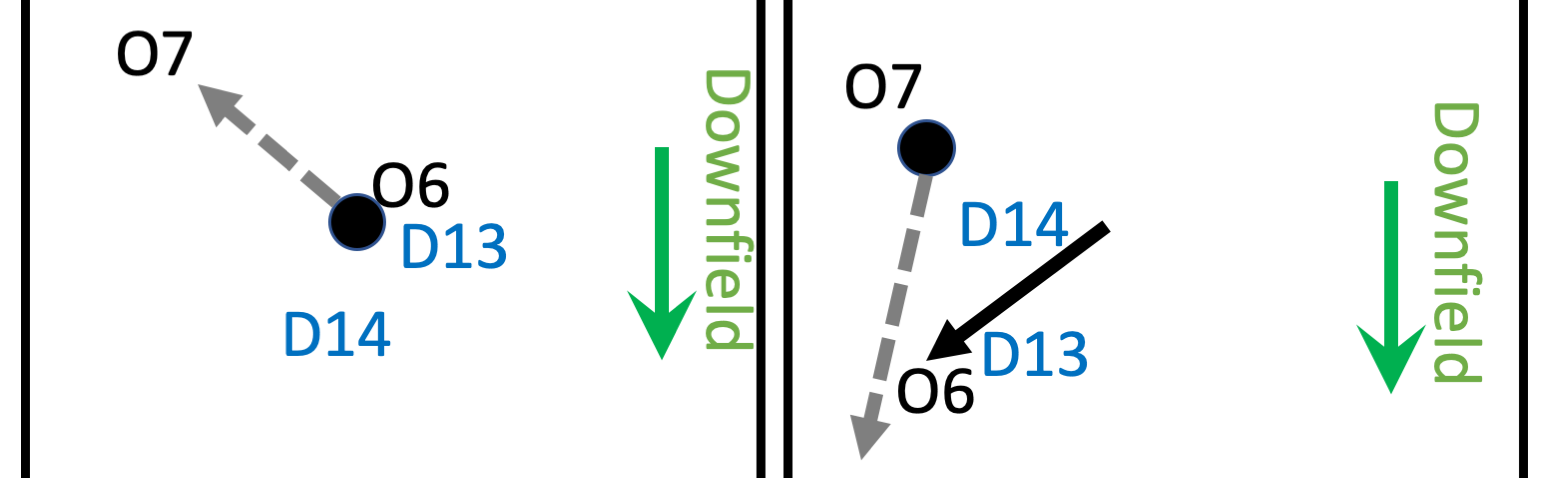
\includegraphics[width=\linewidth]{dump_match_1_45}
 \caption{Person-match: open-side poach countered by 45 degree dump}
 \label{fig:dump_match_1_45}
 \end{marginfigure}
 
O7 positioning back at 45 degrees forces D14 to choose 
whether to poach or match up. 
A poach is easily exploited, 
as in Figure \ref{fig:dump_match_1_45}
where O6 makes a 'give-go' throw (left) then cuts (right) `down the line`, 
taking advantage of the way that D13 is on the wrong side of them 
to prevent the pass back from O7. 
This simple pattern: 
is difficult to stop; 
resets the stall count to zero;
puts O6 in 'power position'\footnote{where, because they are downfield of D13, 
there is no force and they can through 
almost anyway, opening the break side 
and/or making a huck easier.}. 

\begin{marginfigure}%
  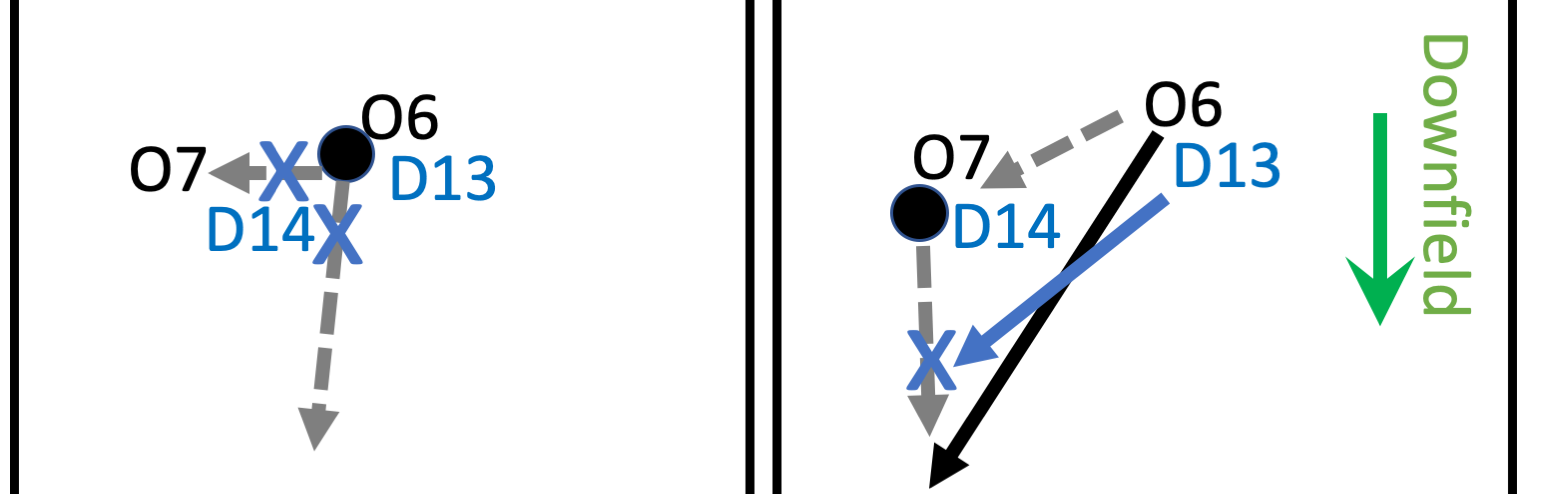
\includegraphics[width=\linewidth]{dump_match_2_45}
 \caption{Person-match: open-side poach, O7 being inline not ideal.}
 \label{fig:dump_match_2_45}
 \end{marginfigure}
 \begin{marginfigure}%
  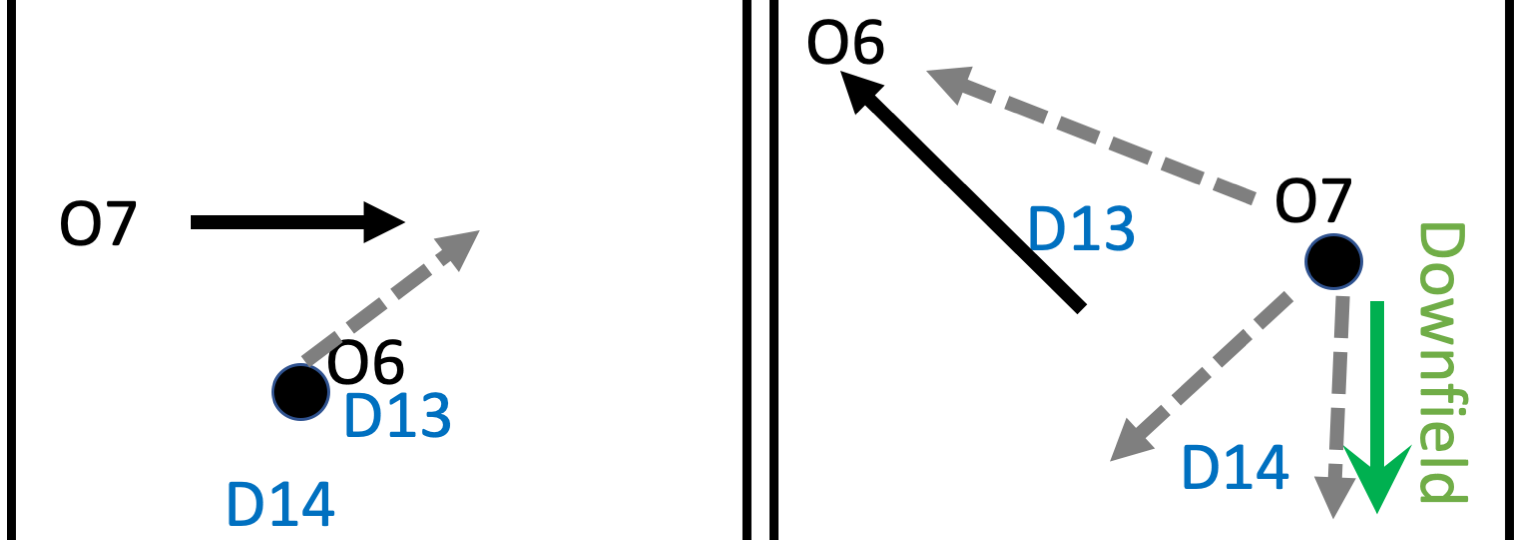
\includegraphics[width=\linewidth]{dump_match_3_45}
 \caption{Person-match: open-side poach, attack the break side.}
 \label{fig:dump_match_3_45}
 \end{marginfigure}
Figure \ref{fig:dump_match_2_45} (left), however, 
shows how if O7 stands further downfield 
D14 might cover O7 AND 
limit throws from O6 to others downfield. 
Even if O6 gets it to O7, 
(Figure \ref{fig:dump_match_2_45} (right)), 
the give-go may be more challenging because 
D14 is amongst the action 
and the angles are less favourable. 
Figure \ref{fig:dump_match_3_45} shows 
another variation 
where O7 crosses behind 
to the break side, 
opening the whole field 
(as long as O6 gets out of the way) 
 or a pass back to O6 to 
 keep things moving. 

\begin{marginfigure}%
  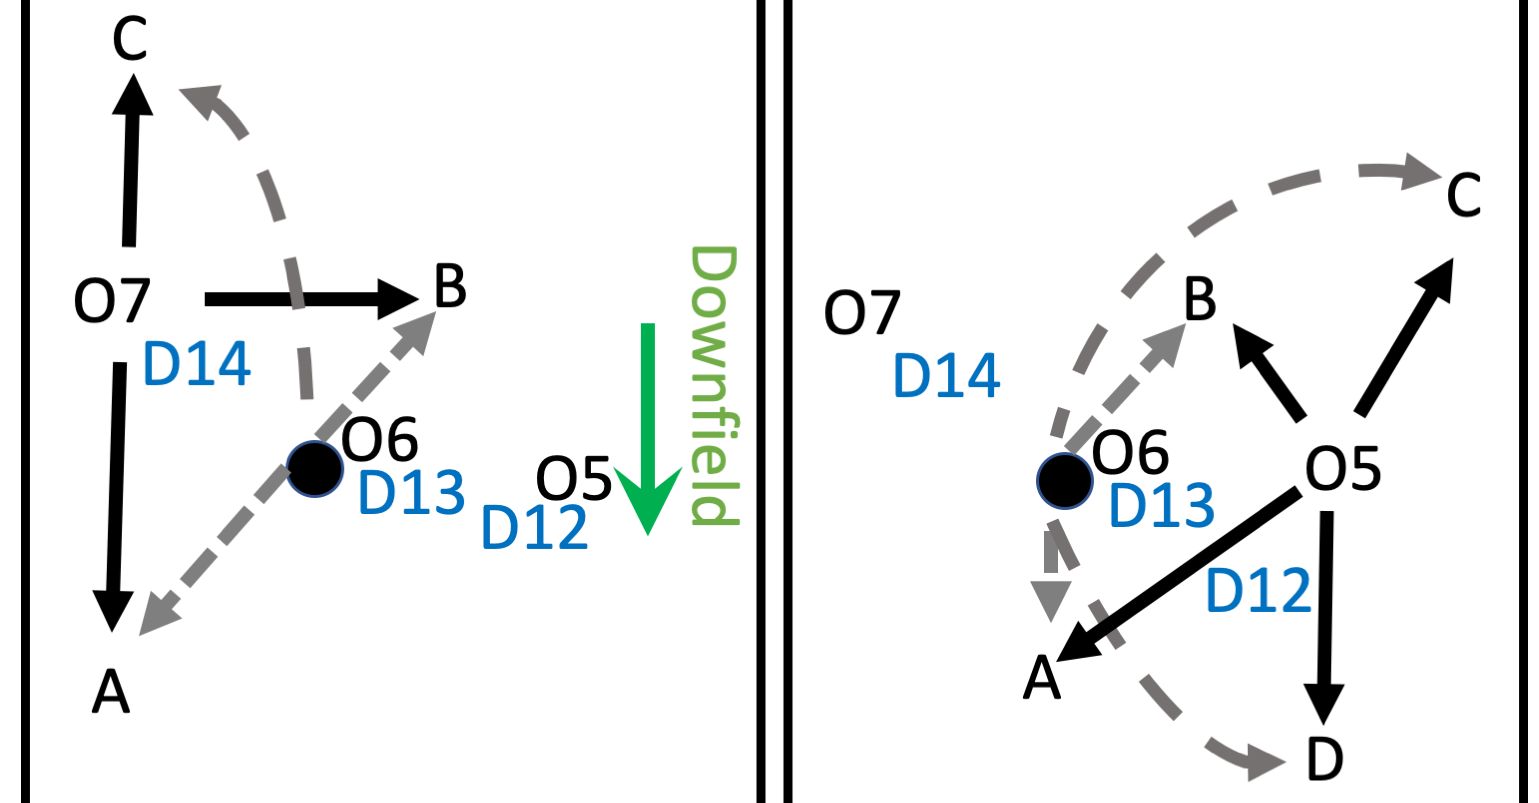
\includegraphics[width=\linewidth]{dump_match_4_tight}
 \caption{Person-match: tighter defence, open-side (left) or break-side (right) dumps.}
 \label{fig:dump_match_4_tight}
 \end{marginfigure}

\newthought{Variations 
where defenders are playing person-match}, 
rather than defending space are shown in Figure \ref{fig:dump_match_4_tight}. 
In each O6 has multiple options to
throw to, with: A putting O5 or O7 into power position;
and B and C potentially opening the break side. 
D is probably the hardest throw, but again puts O5 into 
power position. 
D12 and D14 have 3 or 4 places to defend, advantaging offense\footnote{
As well, to get to C first the defenders would need to 
run through / past the receiver, making an intercept 
(without committing a foul) even more difficult.}.  

D12 and D14 cannot see everything at once 
and will likely have to choose between looking mostly 
at the thrower or mostly at the person they are marking. 
One approach to take advantage of this is the (so called) 'feldrunner' 
technique, where if the defender is looking at the thrower (O6) 
the receiver (O5 or O7) simply runs to one of A, B, C or D 
and O6 throws it to them.  
Alternatively, if the defender is looking at O5/7, 
O6 simply throws a soft pass to A, B, C or D that 
O5 or O7 can run onto.  
Importantly this 
tends to work better if the dump(s)
(O5 and/or O7) are stationary until 
the thrower (O6) has 'engaged the dump' 
and is no longer looking to throw to a cutter downfield. 
And 'engaging the dump' tends to work better 
if you do it before the stall count gets too high\footnote{1-4 early but great, 
5-6 good, 
7-8 not as good, 
9 possession over,
 huck it downfield for territory instead}. 

\newthought{Takeaways} are: (1) turnovers lose games; 
(2) find the balance between 
maintaining possession and minimising throws taken to score; 
(3) with clean positioning dump throws might have a high completion rate; 
(4) a handler standing at 45 degrees (open side) or level with the disc (break side) 
may give the defence too much to cover. 



%\begin{marginfigure}%
%  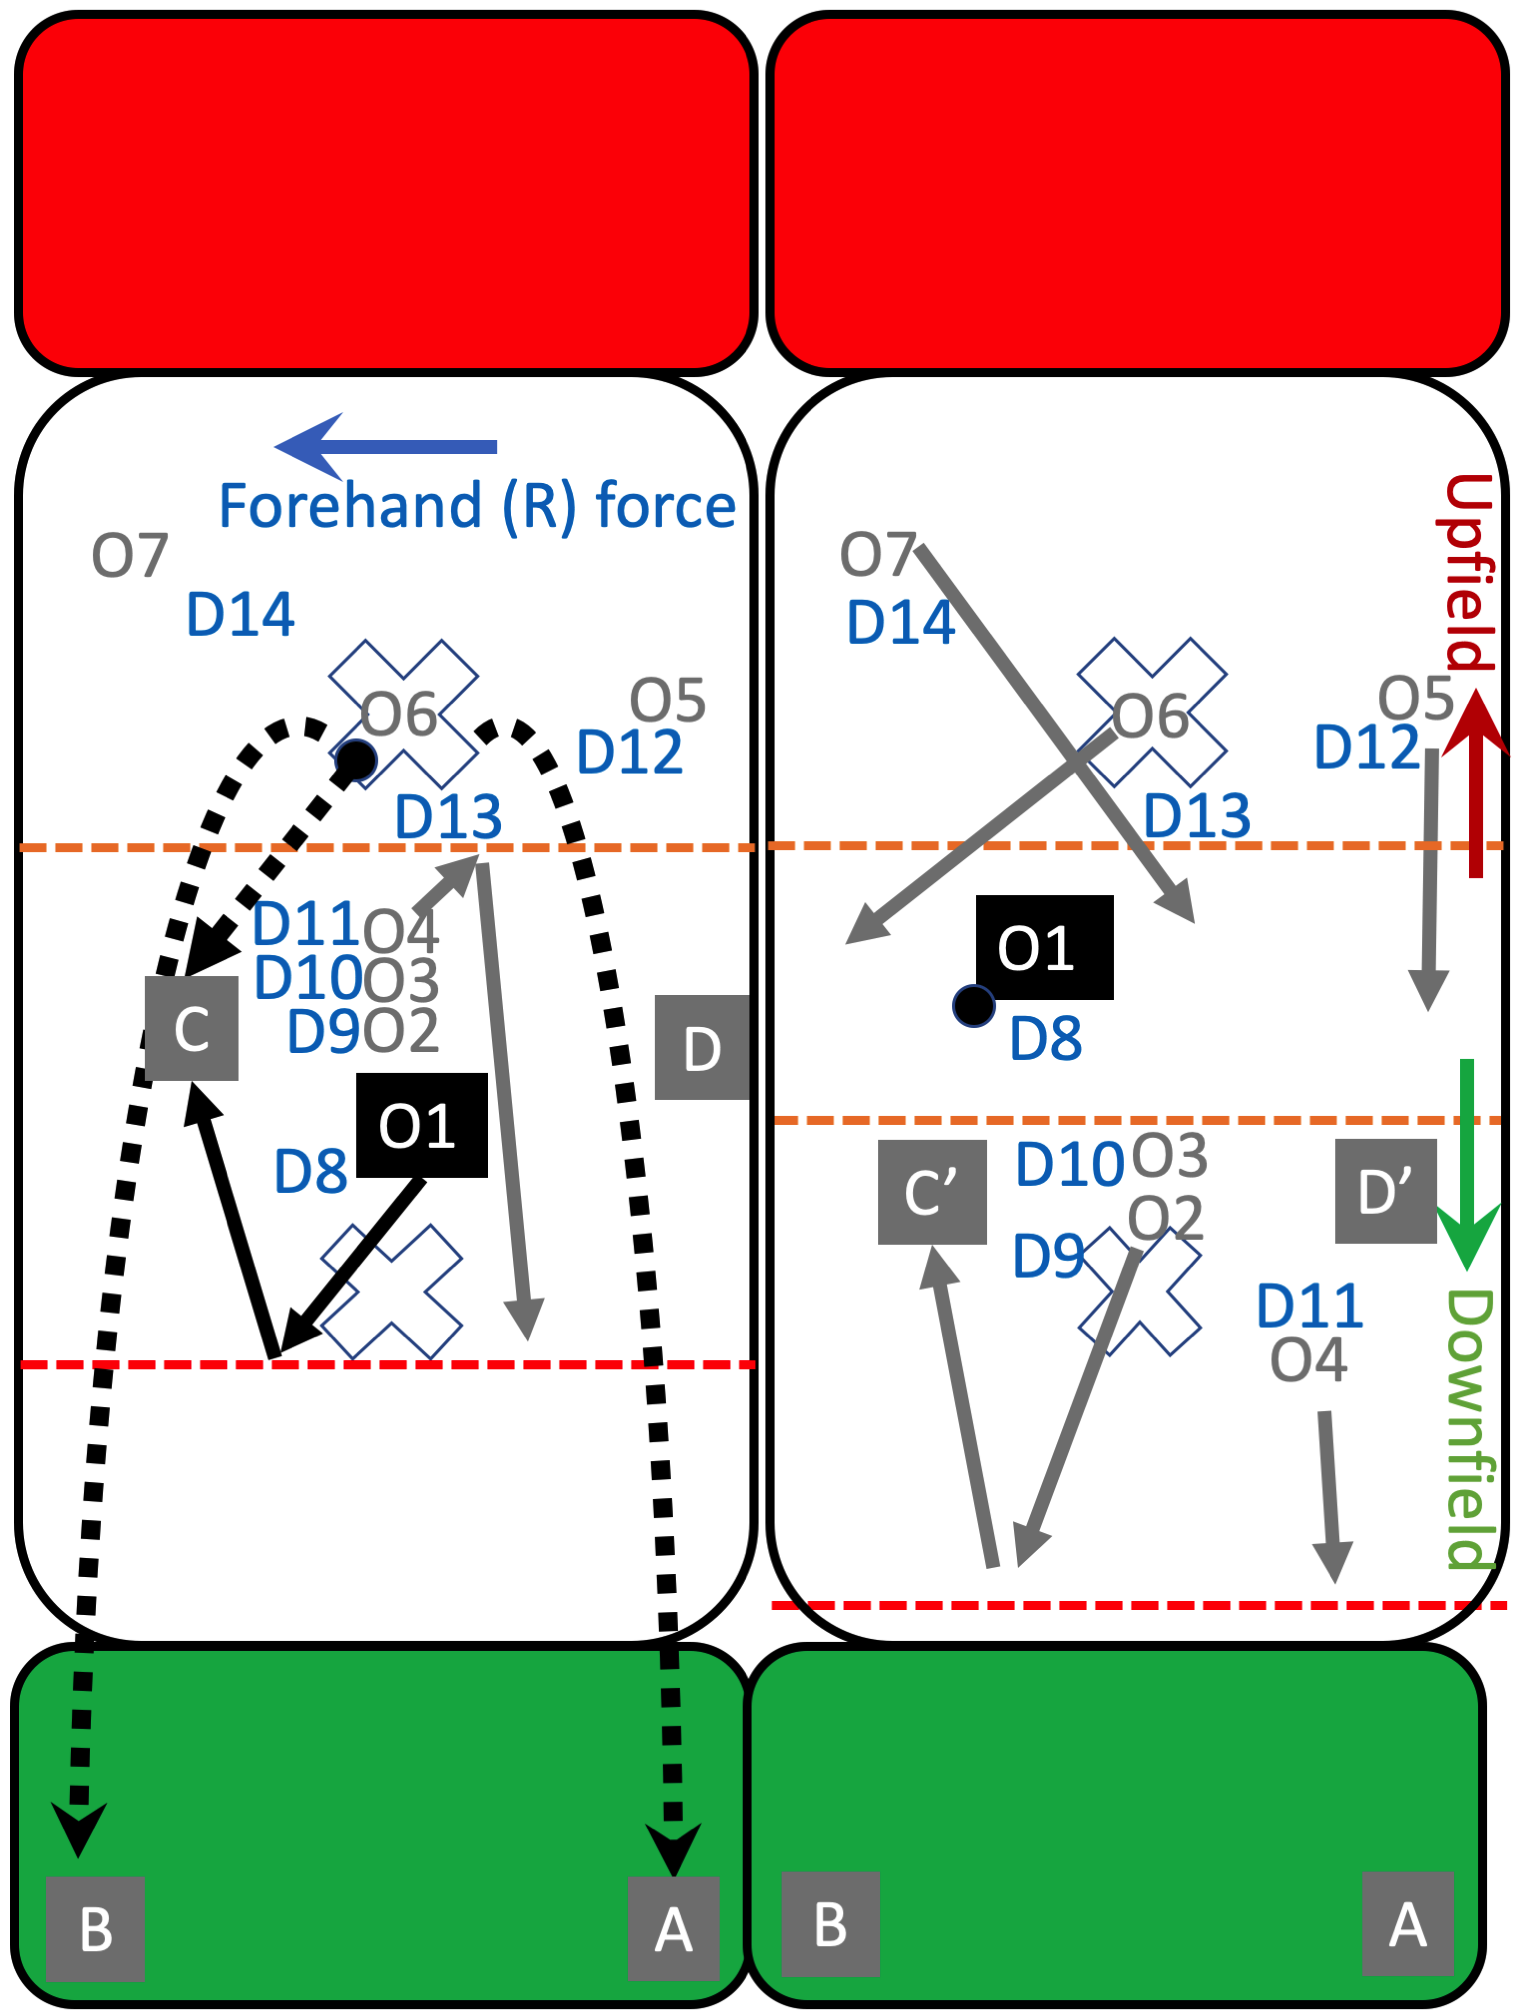
\includegraphics[width=\linewidth]{O1-vertical}
 % \caption{Vertical stack: 
%  starting position (left),
%  and development (right)}
%  \label{fig:O1-vertical}
% \end{marginfigure}


\end{document}
